\section{Diskussion}
\label{sec:Diskussion}

%Der Versuch ist ein Fehler!

Die errechneten Werte für die Schallgeschwindigkeit von $c_\text{Schall,1} = (2,71 \pm 0,02) \cdot 10^{3} \, \frac{\symup{m}}{\symup{s}}$ und $c_\text{Schall,2} = (2,71 \pm 0,03) \cdot 10^{3}$ $\frac{\symup{m}}{\symup{s}}$
liegen beide im Rahmen der Literaturwerte von $c_\text{Acryl} = 2670$ bis $2760$ $\frac{\symup{m}}{\symup{s}}$\cite{acryl}.
Da beide Werte auch eine ähnliche Standardabweichung aufweisen, scheinen beide Methode gute Werte zu liefern. Dies ist auch gut an den Plots zu sehen:
Die Messwerte liegen ziemlich genau auf dem jeweiligen Fit.
Es ist jedoch zu beachten, dass die gestapelten Zylinder bei der Impuls-Echo-Methode offensichtlich fehlerhafte Werte geliefert haben, welche in der Rechnung nicht beachtet werden dürfen.

Zur Bestimmung des Abschwächungskoeffizieten $\alpha = (3,1 \pm 0,5)$ $\frac{1}{\symup{m}}$ ist zu bemerken, dass einige Werte ebenfalls weit von der Erwartung abweichen. Diese wurden daher bei der Berechnung nicht beachtet.
Jedoch auch die beachteten Werte weichen verglichen mit der Schallgeschwindigkeitsmessung stark von der Ausgleichsgeraden ab.
Daraus entsteht die vergleichsweise hohe Standardabweichung von circa $16,1 \%$. Auch kann der Wert durch diese starken Schwankungen nicht als genau betrachtet werden.
Der Theoriewert beträgt hier $\alpha_\text{Theorie} = 57$ $\frac{1}{\symup{m}}$, wobei eine starke Abweichung auffällt.

Die Messung selbst gestaltet sich als einfach, da ein statisches System betrachtet wird.

Bei der biometrischen Ausmessung des Augenmodells fällt jedoch auf, dass selbst kleine Veränderungen im Einfallswinkel des Schalls die Form des Graphen stark verändern können.
Ebenfalls wirken sich Reflexionen im Inneren des Modells auf die Form dessen aus. Das Gesamtbild ergibt sich dennoch realitisch mit den äußeren Abmessungen des Modells.

In einem echten Auge nehmen die Augenkammer und die Linse mit je circa $3,6$ mm $\sim \! 16\%$ des gesamten Auges ein.
Der Glaskörper nimmt die restlichen $68 \%$ ein. In dem Modell nimmt die Augenkammer $\sim \! 13\%$ und die Linse $\sim \! 31,5 \%$ ein.
Es fällt auf, dass die Augenkammer ein ähnliches Größenverhätlnis hat, die Linse jedoch circa doppelt so groß ist.
Der Glaskörper nimmt im Modell $\sim \! 55,5 \%$ ein.

Die Abweichungen lassen sich durch die oben beschrieben schnell entstehenden Messfehler erklären.

%Auge       
%Augenkammer  ~3,6mm 
%Linse        ~3,6mm      
%Glaskörper   ~15,18mm    



\section{Anhang}

Hier sind die Graphen aufgeführt.

\begin{figure}
  \centering
  \begin{subfigure}{0.7\textwidth}
    \centering
    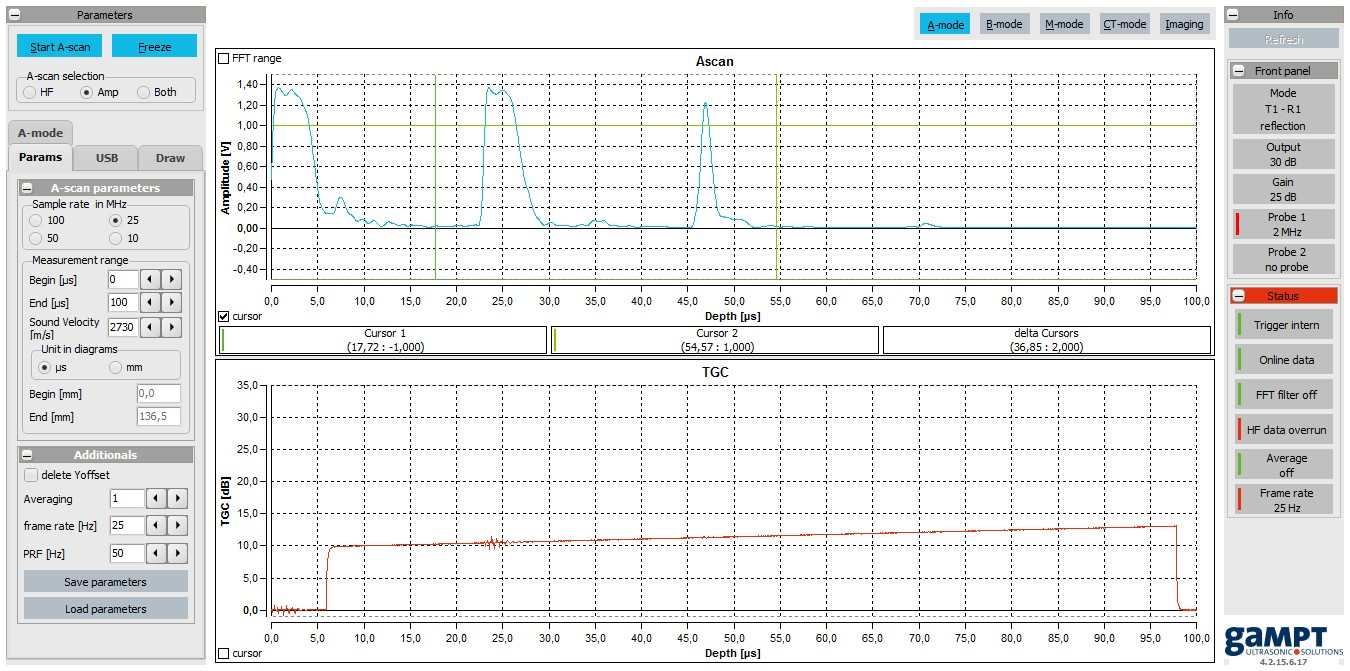
\includegraphics[width=0.95\textwidth]{screens/311.jpg}
    \caption{$d = 3,11$ cm}
    \label{fig:0-deg}
  \end{subfigure}

  \begin{subfigure}{0.7\textwidth}
    \centering
    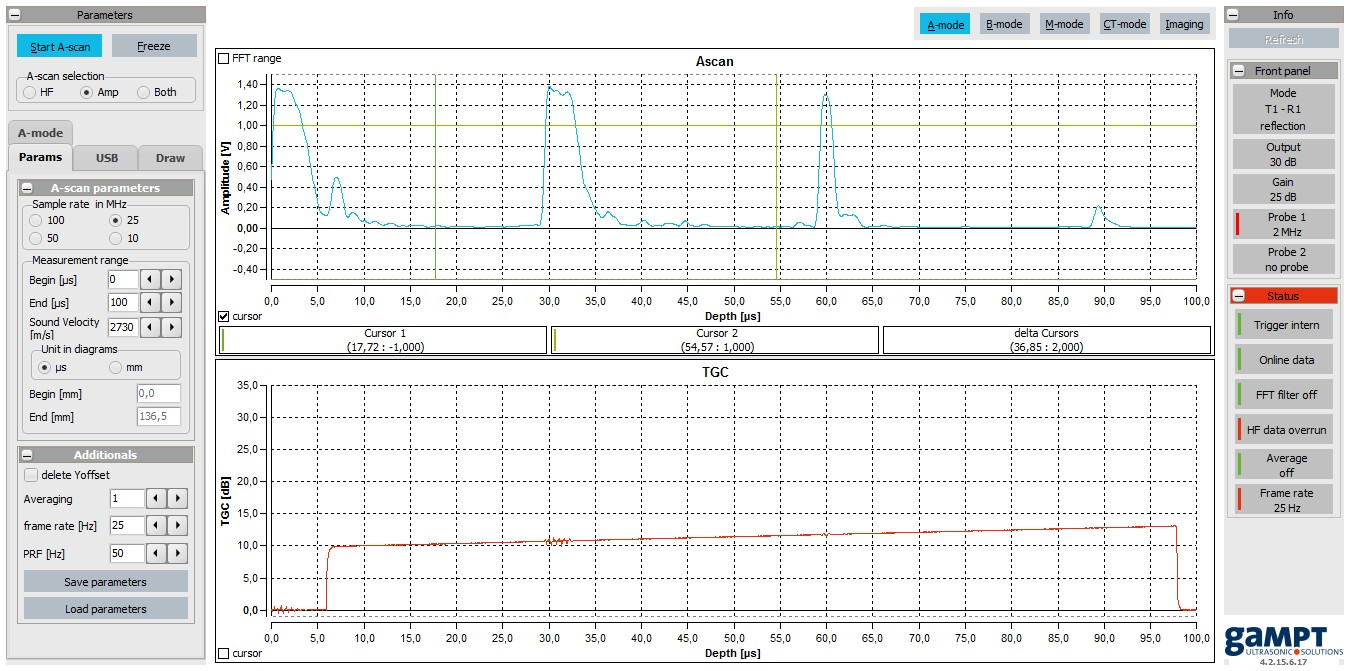
\includegraphics[width=0.95\textwidth]{screens/405.jpg}
    \caption{$d = 4,05°$ cm}
    \label{fig:45-deg}
  \end{subfigure}

  \begin{subfigure}{0.7\textwidth}
    \centering
    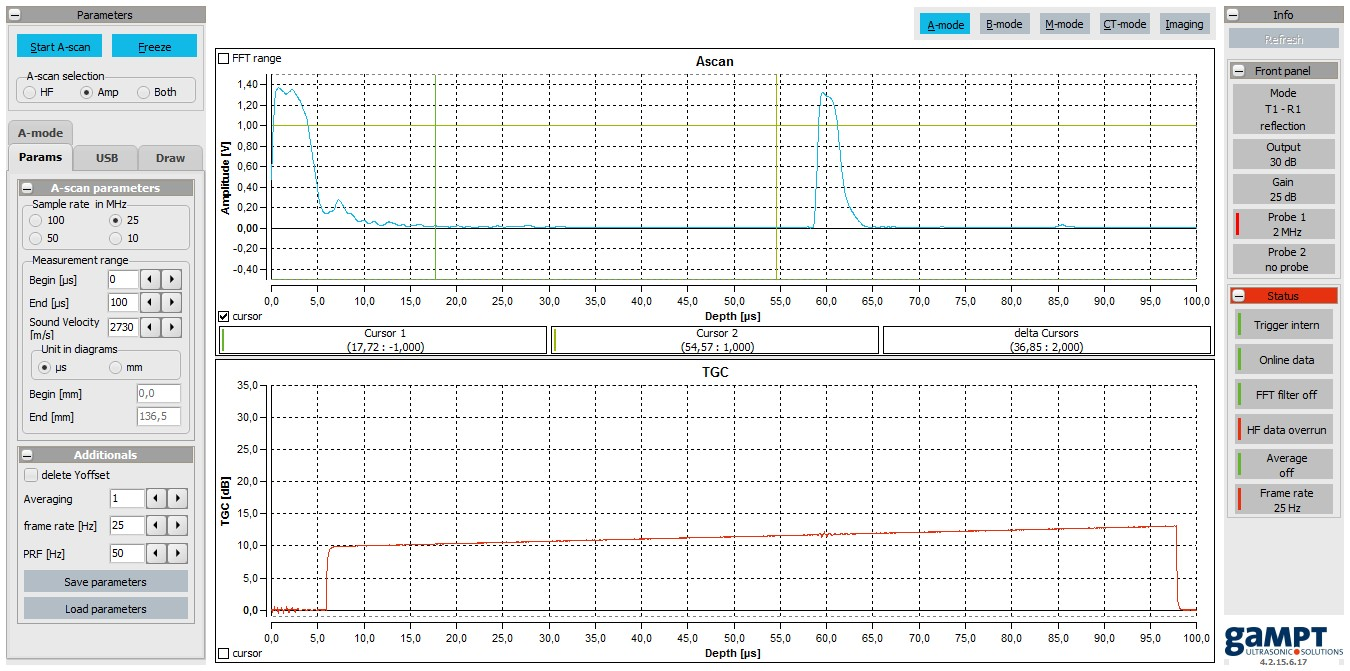
\includegraphics[width=0.95\textwidth]{screens/805.jpg}
    \caption{$d = 8,05°$ cm}
    \label{fig:90-deg}
  \end{subfigure}

  \begin{subfigure}{0.7\textwidth}
    \centering
    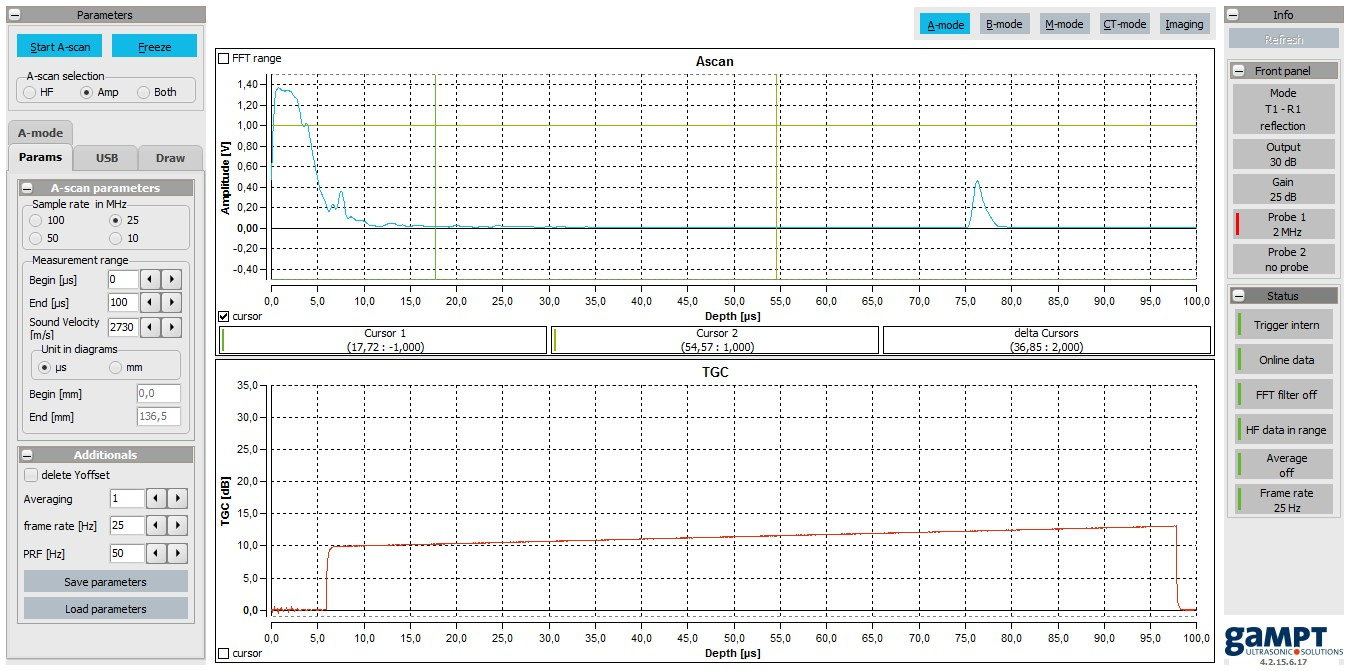
\includegraphics[width=0.95\textwidth]{screens/1021.jpg}
    \caption{$d = 10,21$ cm}
    \label{fig:135-deg}
  \end{subfigure}
  \label{fig: graphen}
\end{figure}


\begin{figure}
  \centering
  \begin{subfigure}{0.7\textwidth}
    \centering
    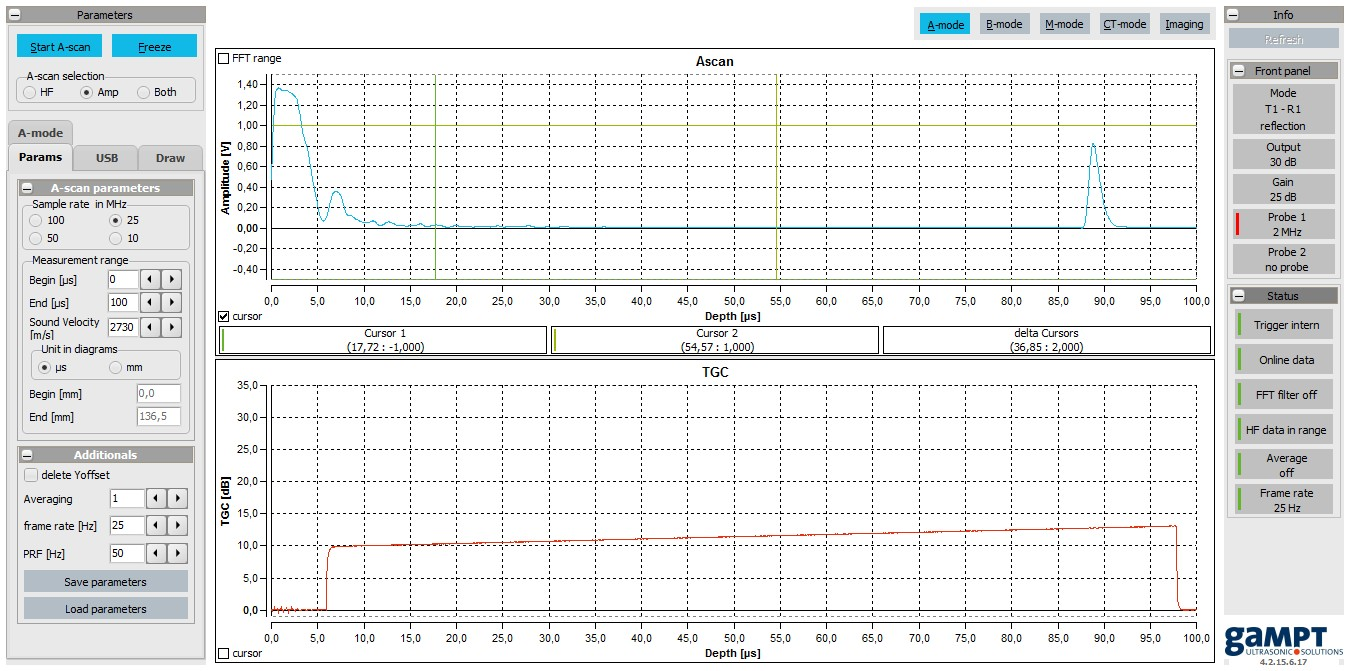
\includegraphics[width=0.95\textwidth]{screens/1205.jpg}
    \caption{$d = 12,05$ cm}
    \label{fig:180-deg}
  \end{subfigure}

  \begin{subfigure}{0.7\textwidth}
    \centering
    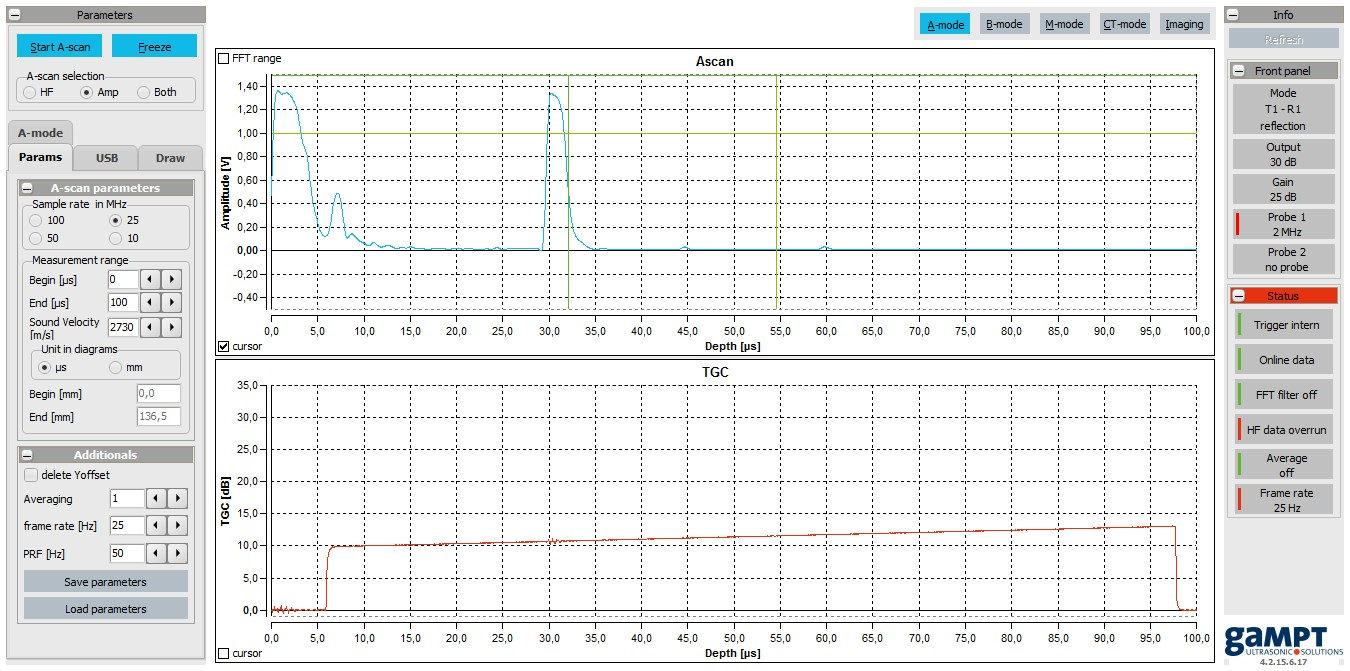
\includegraphics[width=0.95\textwidth]{screens/1610.jpg}
    \caption{$d = 16,10$ cm}
    \label{fig:270-deg}
  \end{subfigure}

  \begin{subfigure}{0.7\textwidth}
    \centering
    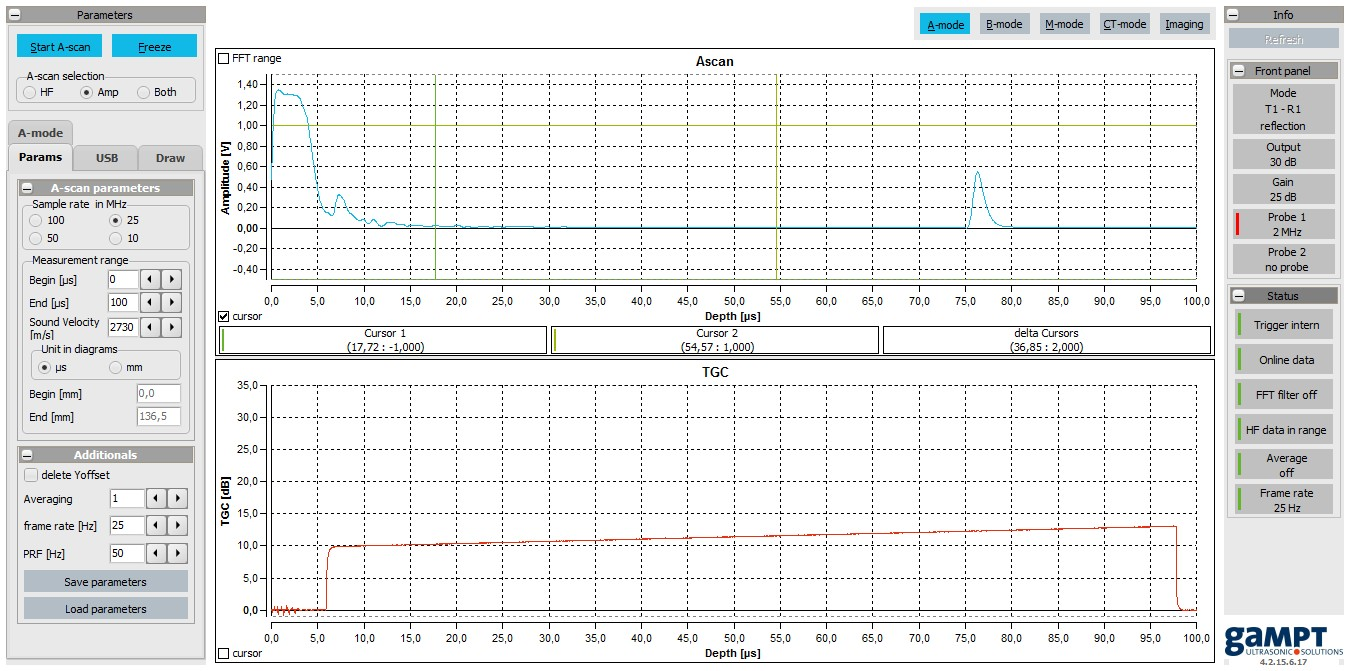
\includegraphics[width=0.95\textwidth]{screens/1826.jpg}
    \caption{$d = 18,26$ cm}
    \label{fig:270-adeg}
  \end{subfigure}
  \caption{Screenshots des Programms bei der Impuls-Echo-Methode.}
  \label{fig: graphen}
\end{figure}



\begin{figure}
  \centering
  \begin{subfigure}{0.7\textwidth}
    \centering
    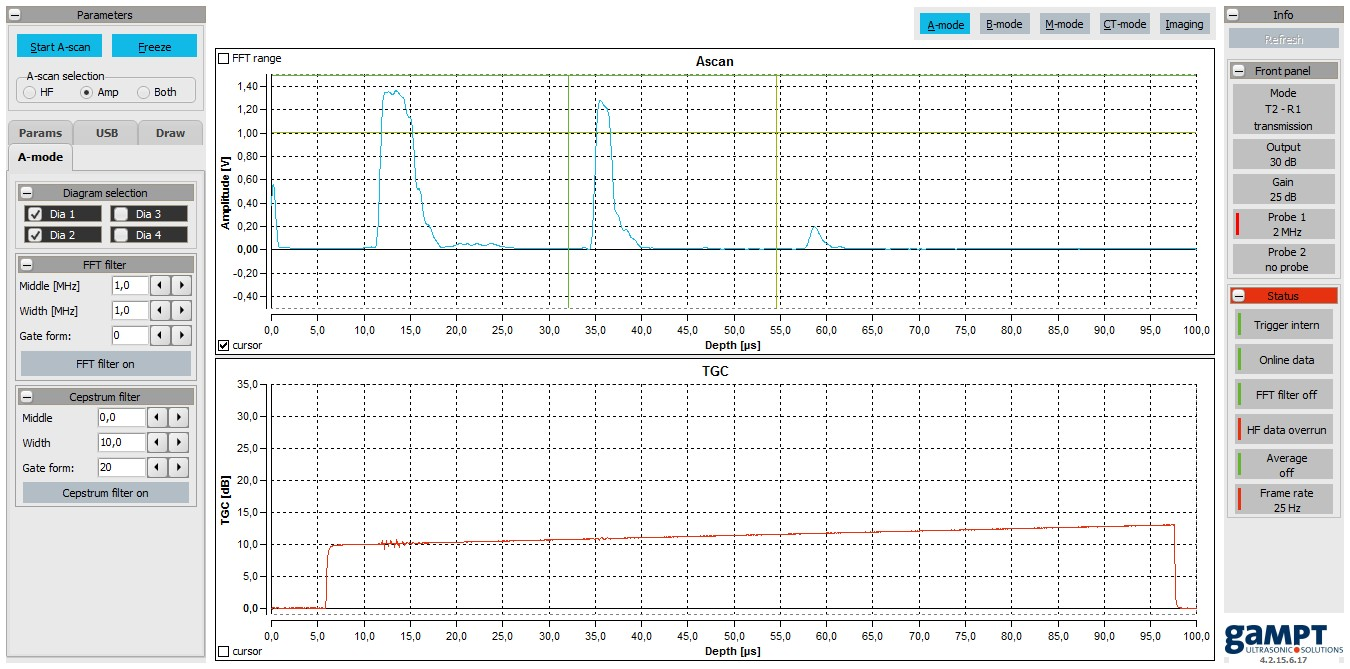
\includegraphics[width=0.95\textwidth]{screens/d311.jpg}
    \caption{$d = 3,11$ cm}
    \label{fig:0-deg}
  \end{subfigure}

  \begin{subfigure}{0.7\textwidth}
    \centering
    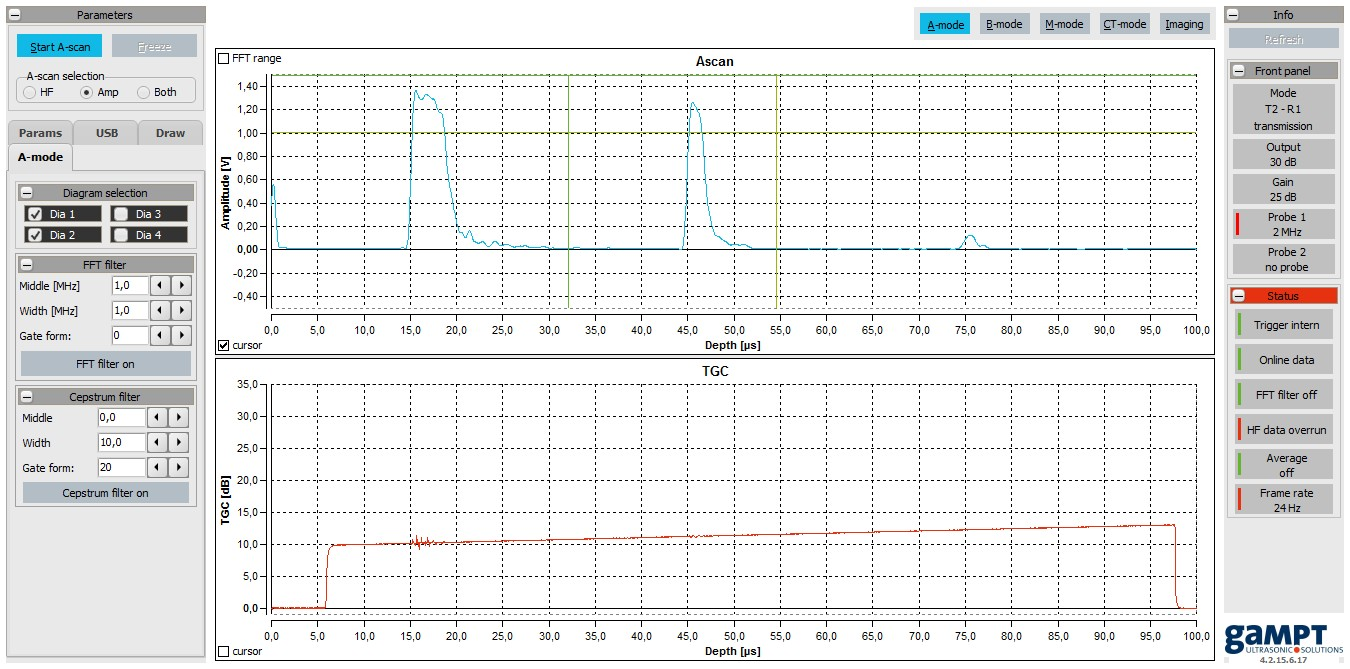
\includegraphics[width=0.95\textwidth]{screens/d405.jpg}
    \caption{$d = 4,05°$ cm}
    \label{fig:45-deg}
  \end{subfigure}

  \begin{subfigure}{0.7\textwidth}
    \centering
    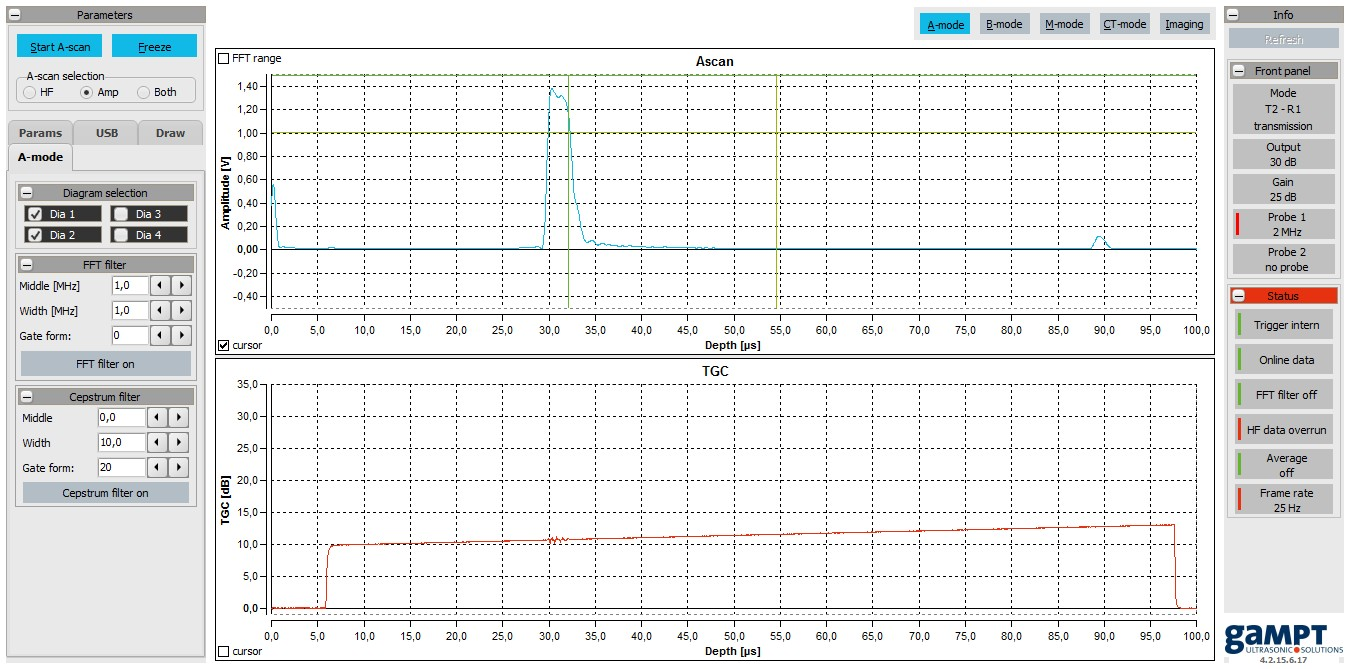
\includegraphics[width=0.95\textwidth]{screens/d805.jpg}
    \caption{$d = 8,05°$ cm}
    \label{fig:90-deg}
  \end{subfigure}

  \begin{subfigure}{0.7\textwidth}
    \centering
    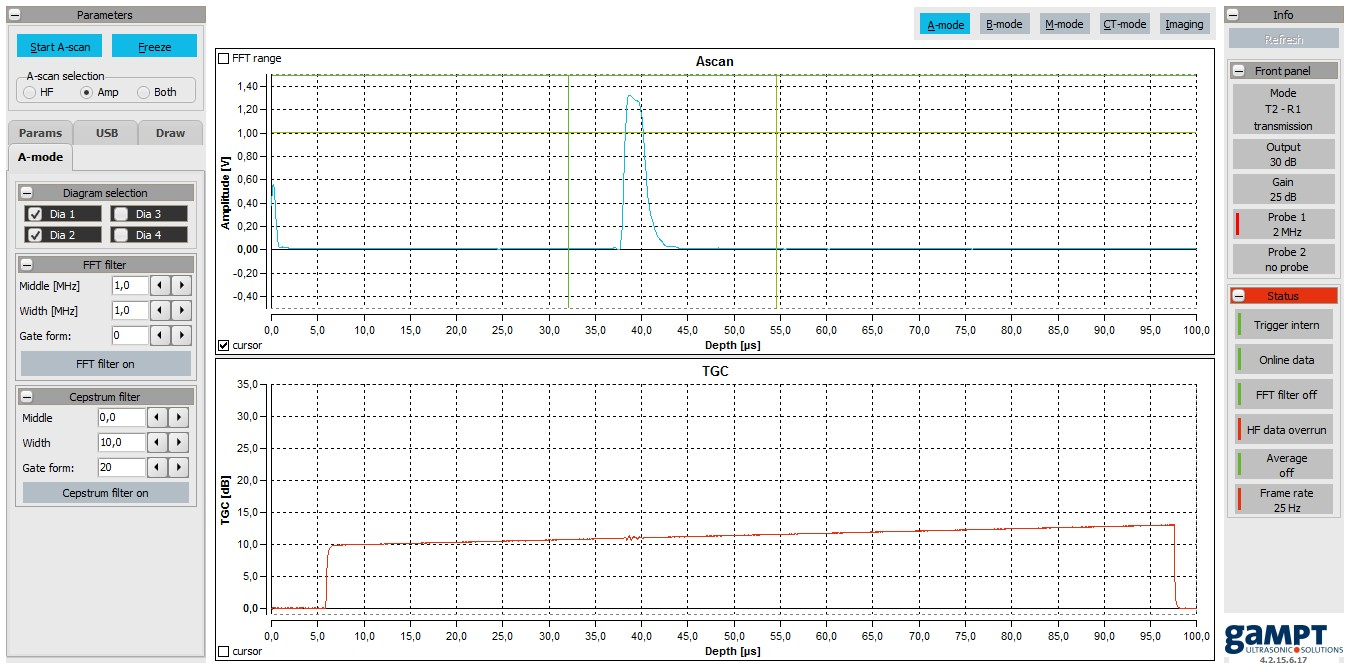
\includegraphics[width=0.95\textwidth]{screens/d1021.jpg}
    \caption{$d = 10,21$ cm}
    \label{fig:135-deg}
  \end{subfigure}

  \label{fig: graphen}
\end{figure}

\begin{figure}
  \centering

  \begin{subfigure}{0.7\textwidth}
    \centering
    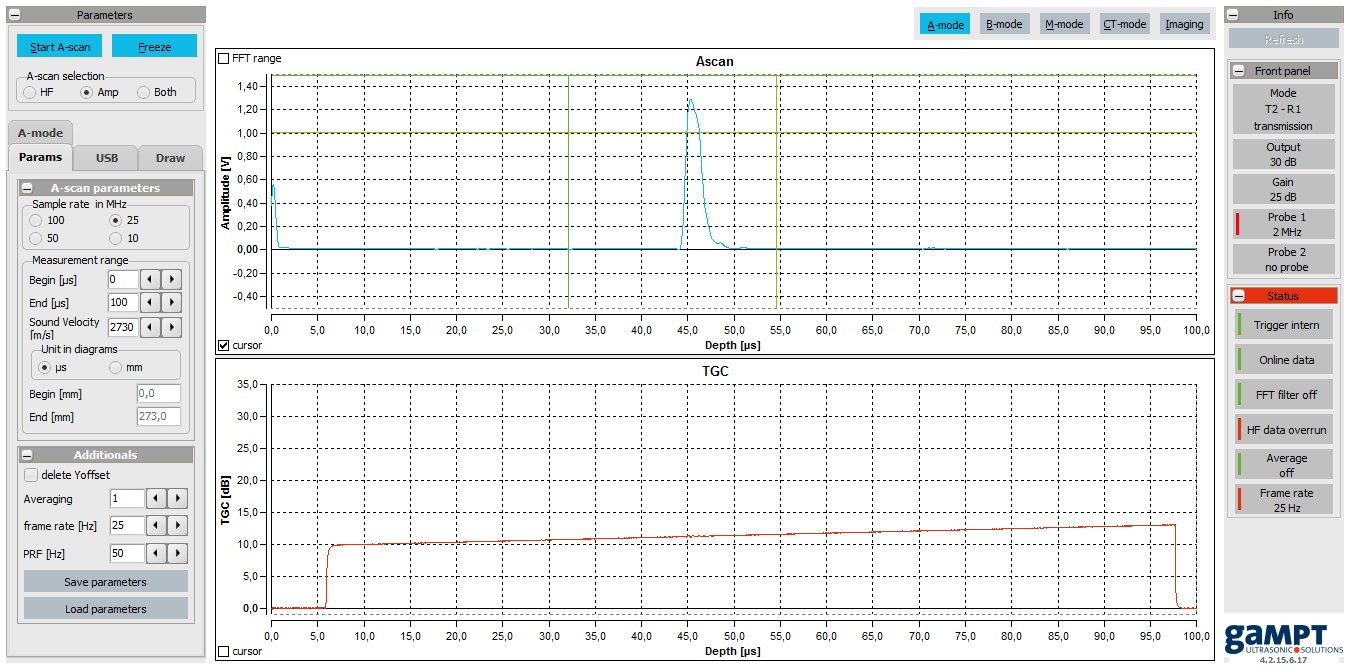
\includegraphics[width=0.95\textwidth]{screens/d1205.jpg}
    \caption{$d = 12,05$ cm}
    \label{fig:180-deg}
  \end{subfigure}
  \caption{Screenshots des Programms bei der Durchschall-Methode.}
  \label{fig:durchgraphen}
\end{figure}

\begin{figure}
    \centering
    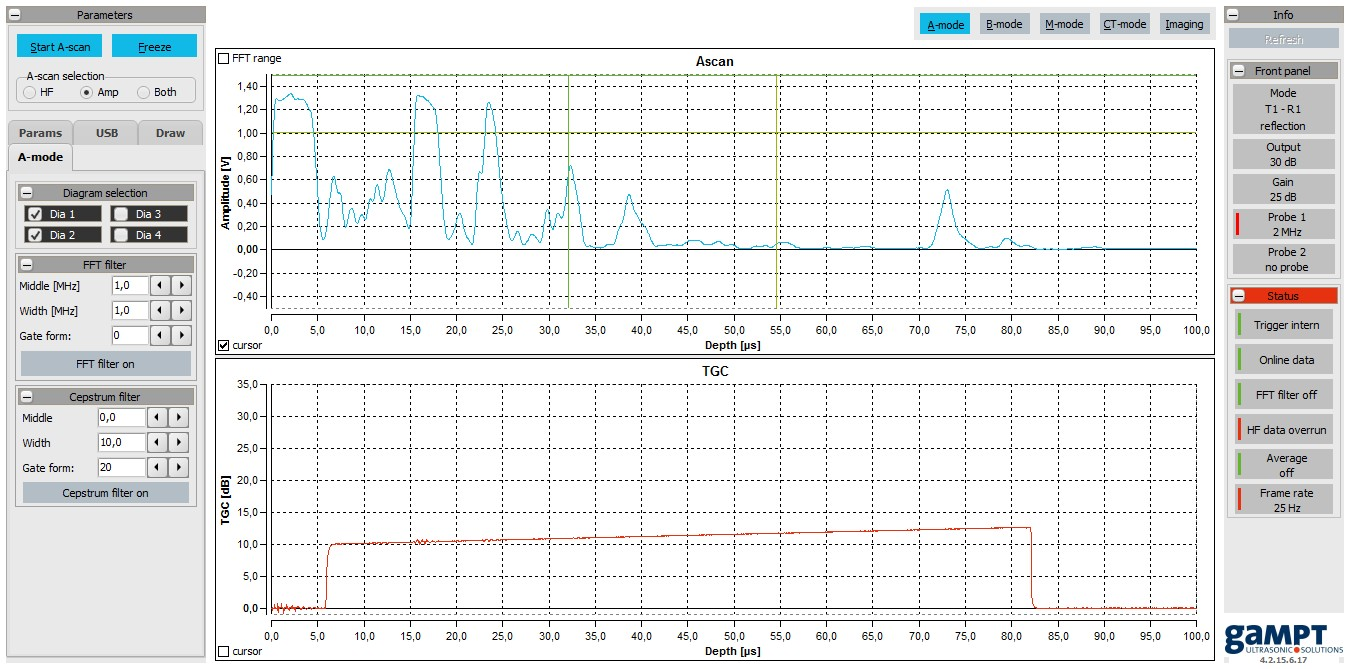
\includegraphics[width=0.7\textwidth]{screens/auge.jpg}
    \caption{Screenshot des Programms bei der Vermessung des Augenmodells.}
    \label{fig:screenauge}
\end{figure}